\subsection{Descriptions}
A common source NMOS amplifier is constructed for DC and small-signal analysis.

\FloatBarrier

\begin{figure}[h!]
	\centering
	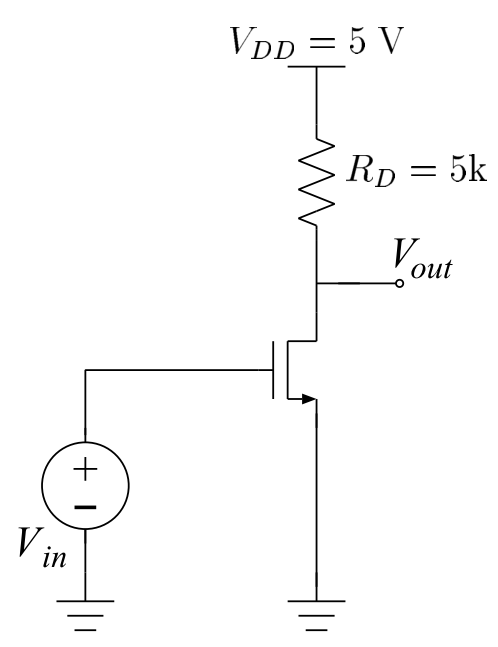
\includegraphics[scale=0.75]{./images/circuit_2.PNG}
	\caption{Common-Source Amplifier}
	\label{fig:circuit_2}
\end{figure}

\FloatBarrier

$V_{in}$ or $V_{GS}$ is swept from $0$ \si{\volt} to $3$ \si{\volt} in increments of $0.1$ \si{\volt} and $V_{out}$ or $V_{DS}$ is measured at each point.
This range is chosen in order to capture the full range of the saturation operating mode and the transition from saturation to triode mode of the NMOS in the VTC.
The results are plotted and tabulated below. \\

The circuit is then biased at $V_{in(eq2)}$ in the middle of the saturation region and a sine wave with $10$ \si{\milli\volt} amplitude and $1$ \si{\mega\hertz} is applied at the input. Note, for the measurement taken at $1$ \si{\mega\hertz}, a $30$ \si{\milli\volt} amplitude is used for the input sine wave because the original $10$ \si{\milli\volt} amplitude is too weak and yields a heavily distorted output signal that is immeasureable with the oscilloscope. The DC bias of the circuit is then increased by $10$ \si{\milli\volt}, and the experiment is repeated. The small-signal gain values can be found in tables (\ref{tab:gain_part2}) and (\ref{tab:gain_part2_plus}).

\subsection{Calculations}

\FloatBarrier

\begin{table}[h!]
	\centering
	\caption{Figure (\ref{fig:part2_vtc}) Data}
	\label{tab:part2_vtc}
	\csvautotabular{./tables/sim2_vtc.csv}
\end{table}

\FloatBarrier

To find the DC voltage at the middle of saturation region $V_{in(eq2)}$, the average from the highest and lowest $V_{out}$ value in the VTC is calculated.
Then, and the closest value of $V_{in}$ that corresponds to the the calculated average is the value taken for $V_{in(eq2)}$. \\

\begin{equation}
	\label{eq:v_in_eq2}
	\frac{5 V + 0.439 V}{2} = 2.720 V \approx V_{out} = 2.602 V \Rightarrow V_{in(eq2)} = 2.3 V
\end{equation}

The amplitude of the output sine wave is measured for each input sine wave. 
From the output amplitudes, the small signal gain in $\frac{V}{V}$ is found for each frequency.

\FloatBarrier

\begin{table}[h!]
	\centering
	\caption{Gain of Common Source Amplifier}
	\label{tab:gain_part2}
	\csvautotabular{./tables/gain_part2.csv}
\end{table}

\FloatBarrier

\begin{table}[h!]
	\centering
	\caption{Gain of Common Source Amplifier with $10$ \si{\milli\volt} Higher Bias}
	\label{tab:gain_part2_plus}
	\csvautotabular{./tables/gain_part2_plus10mV.csv}
\end{table}

\FloatBarrier

\subsection{Analysis}

\FloatBarrier

\begin{figure}[h!]
	\centering
	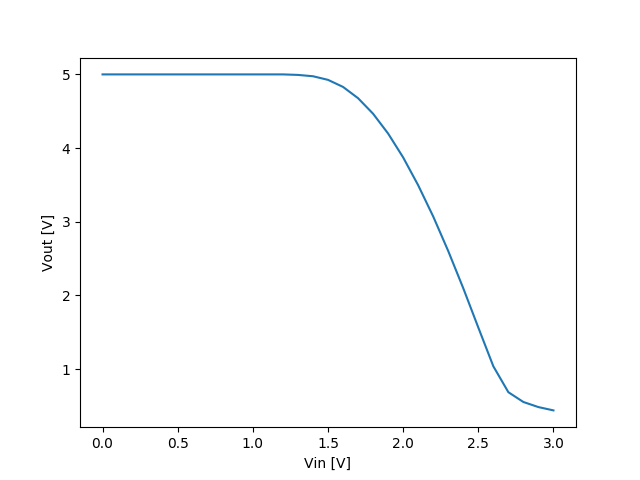
\includegraphics[scale=0.75]{./images/sim2_vtc.PNG}
	\caption{VTC of Common-Source NMOS Amplifier}
	\label{fig:part2_vtc}
\end{figure}

\FloatBarrier

From the VTC in Figure (\ref{fig:part2_vtc}), the NMOS begins and remains in cutoff until $V_{in} = 1.3$ \si{\volt} where $V_{out}$ begins to dip below $V_{DD}$.
The NMOS then enters the saturation region and remains there until the slope of the curve begins to decrease at around $V_{in} = 2.6$ \si{\volt}.
Beyond that point, the NMOS operates in triode mode. \\

\FloatBarrier

\begin{figure}[h!]
	\centering
	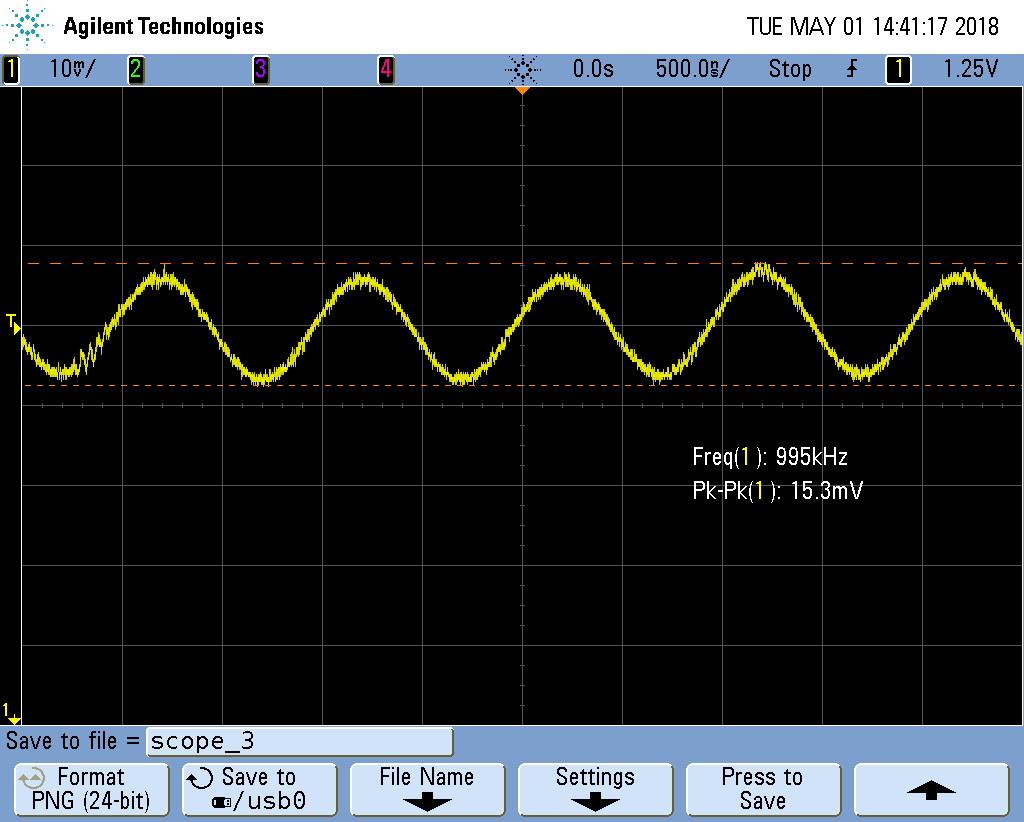
\includegraphics[scale=0.3]{./images/SCOPE_3.PNG}
	\caption{Output Voltage Sine Wave, 1 \si{\mega\hertz}}
	\label{fig:1mhz_original}
\end{figure}

\FloatBarrier

This experiment is repeated with sine waves with varying frequencies.

\FloatBarrier

\begin{figure}[h!]
	\centering
	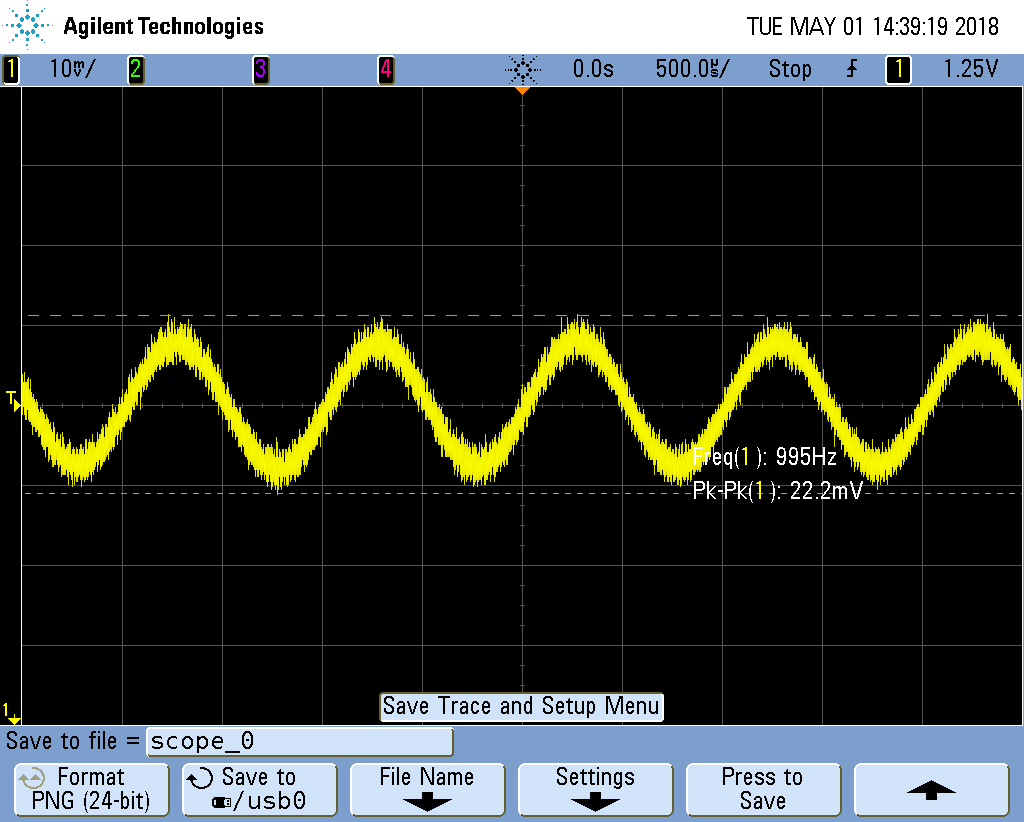
\includegraphics[scale=0.3]{./images/SCOPE_0.PNG}
	\caption{Output Voltage Sine Wave, 1 \si{\kilo\hertz}}
	\label{fig:1khz_original}
\end{figure}

\FloatBarrier

\begin{figure}[h!]
	\centering
	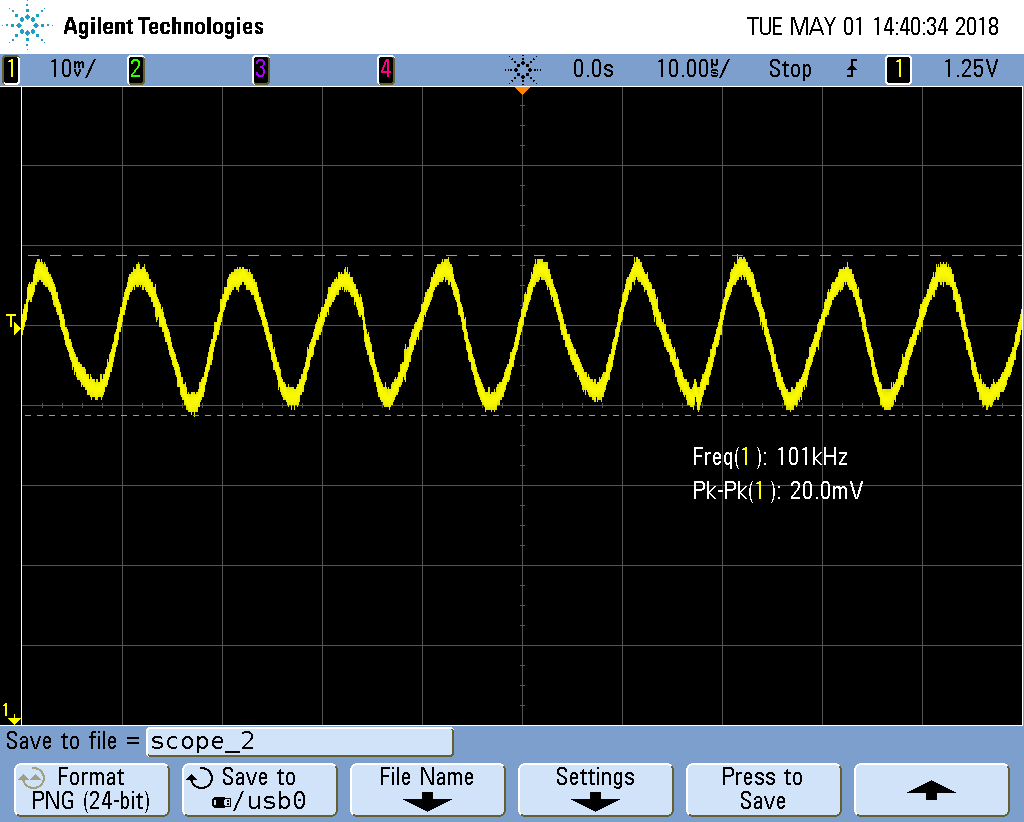
\includegraphics[scale=0.3]{./images/SCOPE_2.PNG}
	\caption{Output Voltage Sine Wave, 100 \si{\kilo\hertz}}
	\label{fig:100khz_original}
\end{figure}

\FloatBarrier

The small signal gain is observed to decrease as the frequency increases.
This is expected because parasitic capacitances in the NMOS cause the circuit to effectively behave like a low-pass filter. \\

\FloatBarrier

\begin{figure}[h!]
	\centering
	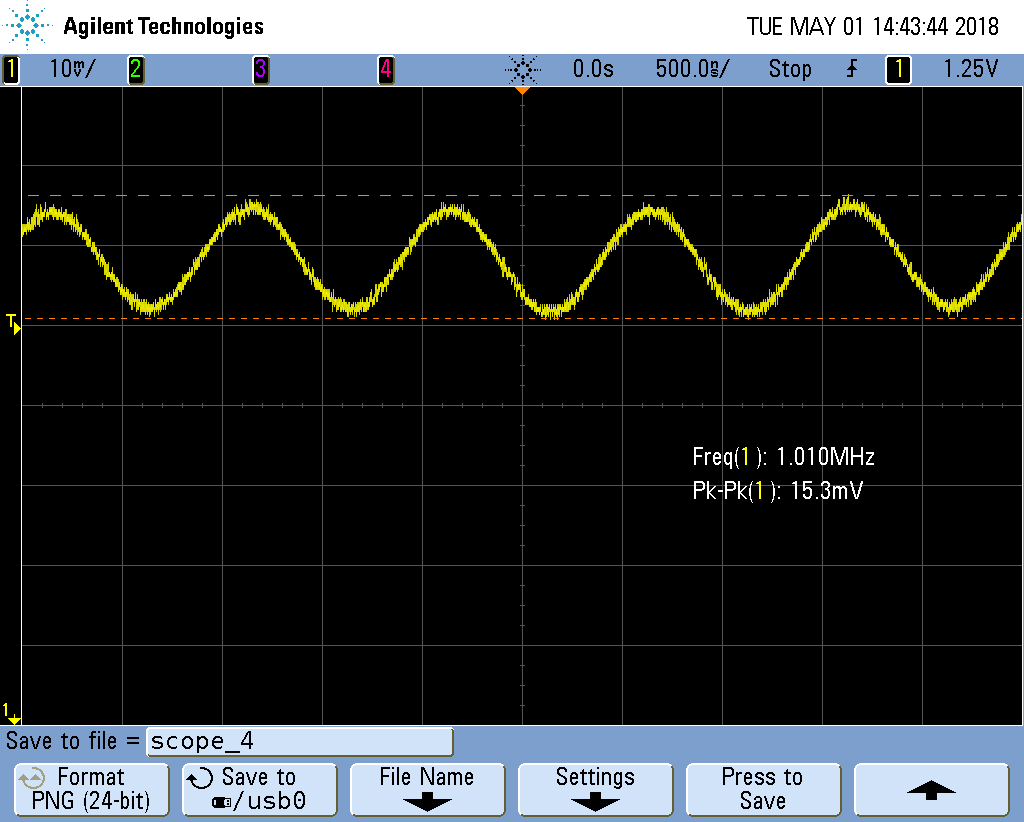
\includegraphics[scale=0.3]{./images/SCOPE_4.PNG}
	\caption{Output Voltage Sine Wave, 1 \si{\mega\hertz}, Increased DC Bias}
	\label{fig:1mhz_original}
\end{figure}

\FloatBarrier

\begin{figure}[h!]
	\centering
	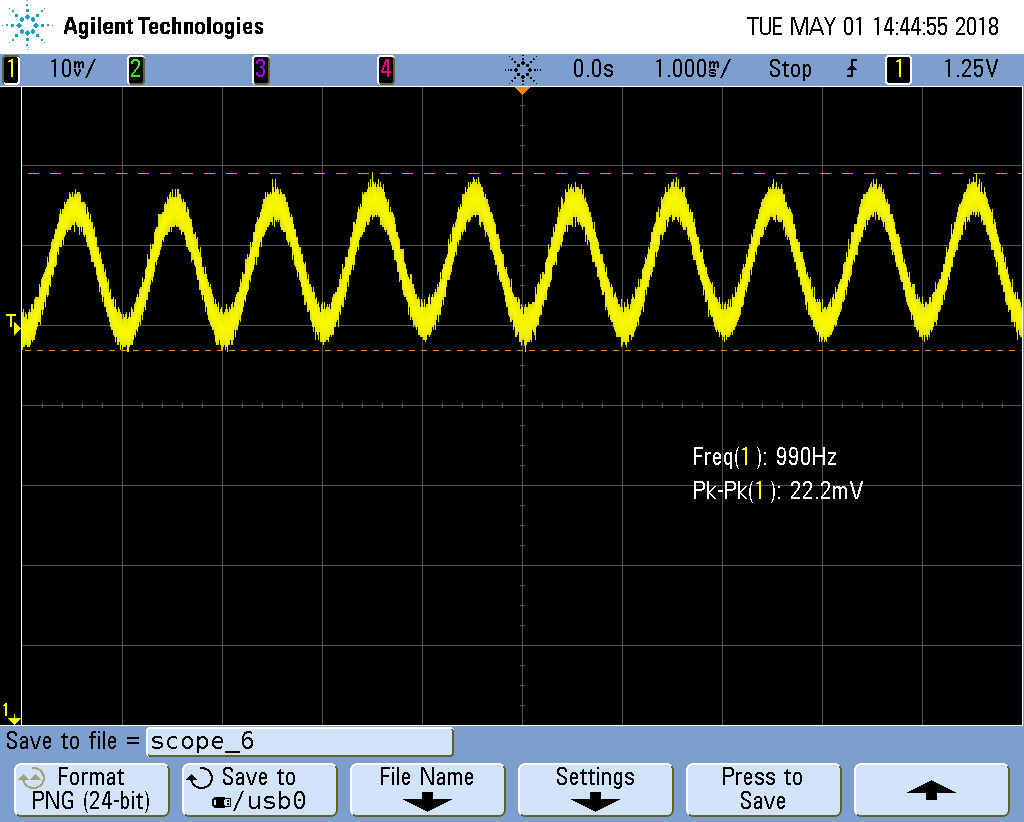
\includegraphics[scale=0.3]{./images/SCOPE_6.PNG}
	\caption{Output Voltage Sine Wave, 1 \si{\kilo\hertz}, Increased DC Bias}
	\label{fig:1khz_original}
\end{figure}

\FloatBarrier

\begin{figure}[h!]
	\centering
	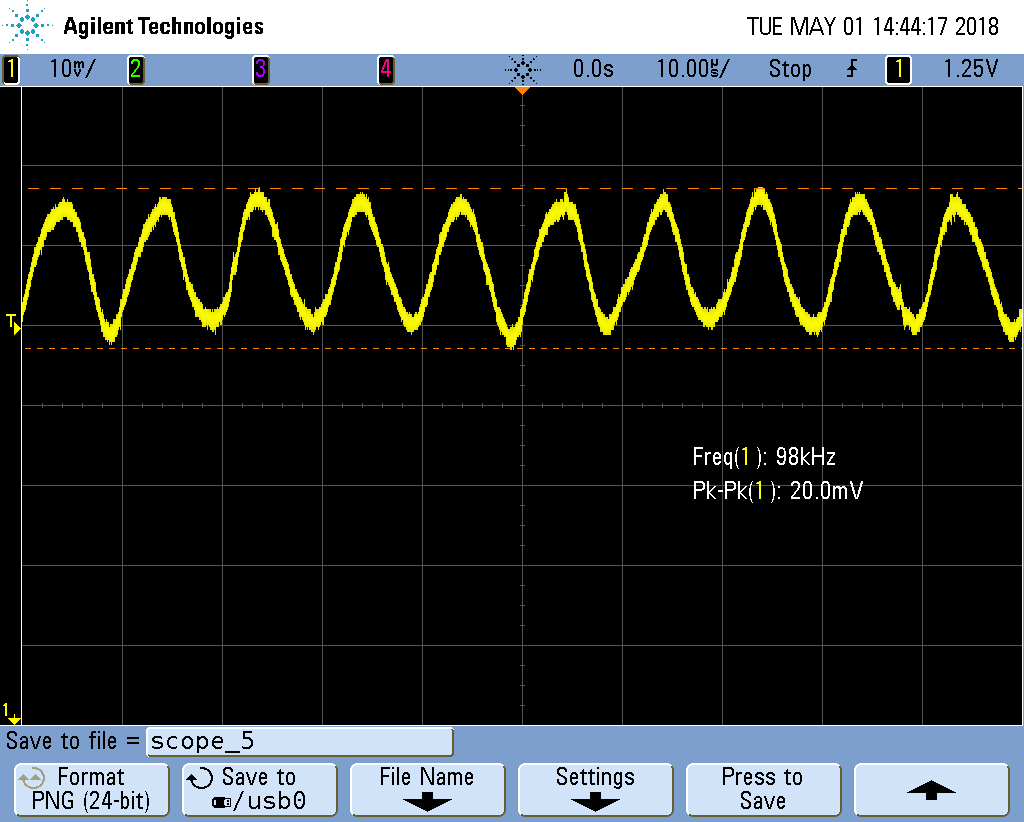
\includegraphics[scale=0.3]{./images/SCOPE_5.PNG}
	\caption{Output Voltage Sine Wave, 100 \si{\kilo\hertz}, Increased DC Bias}
	\label{fig:100khz_original}
\end{figure}

\FloatBarrier

As expected, the new gain values are slightly higher than the values found for the original DC bias.
This is because in saturation mode, $V_{out}$ is directly proportional to the drain current, which is directly proportional to the square of $V_{in}$. This means that as $V_{in}$ increases in the saturation region, the slope of the VTC $\frac{dV_{out}}{dV_{in}}$, another definition for the small-signal gain, increases as well. \\
